\section{Anhang}
\begin{figure}[H]
    \centering
    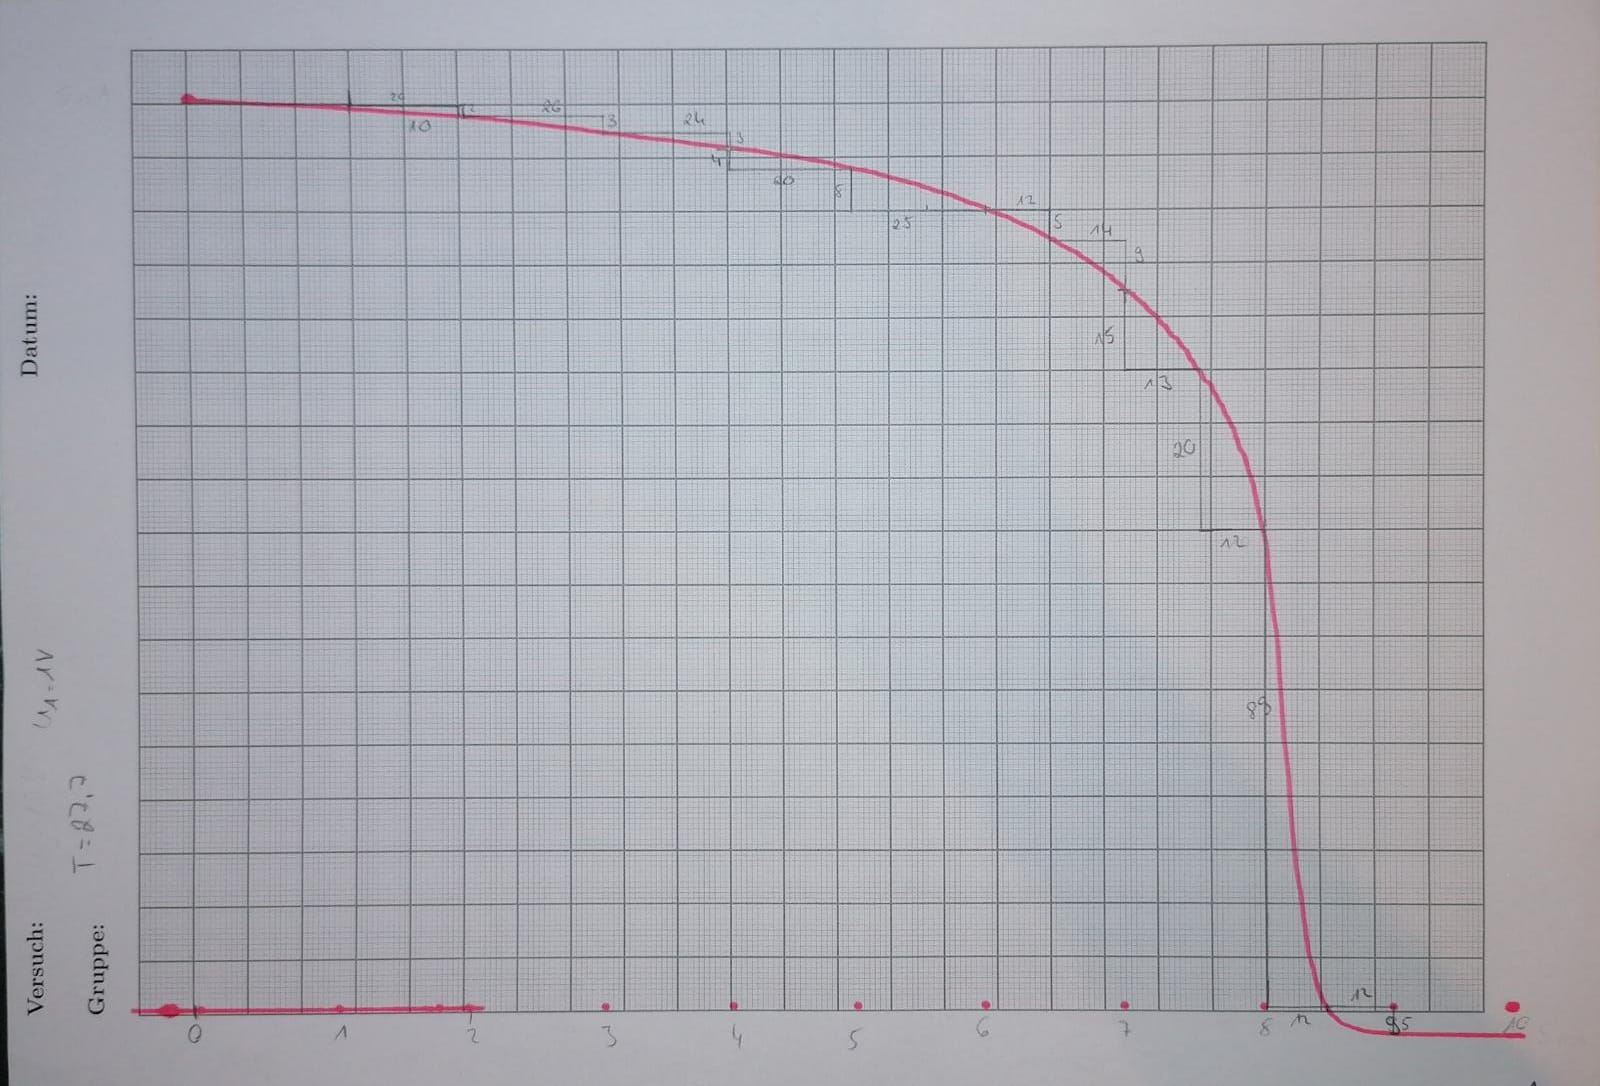
\includegraphics[scale=0.25]{content/Kurve27.jpg}
    \caption{Aufgenommene Messwerte bei $T = 27.7\unit{\degreeCelsius}$ und einer Bremspannung von $U_A = \qty{1}{V}$.}
    \label{fig:27}
\end{figure}

\begin{figure}[H]
    \centering
    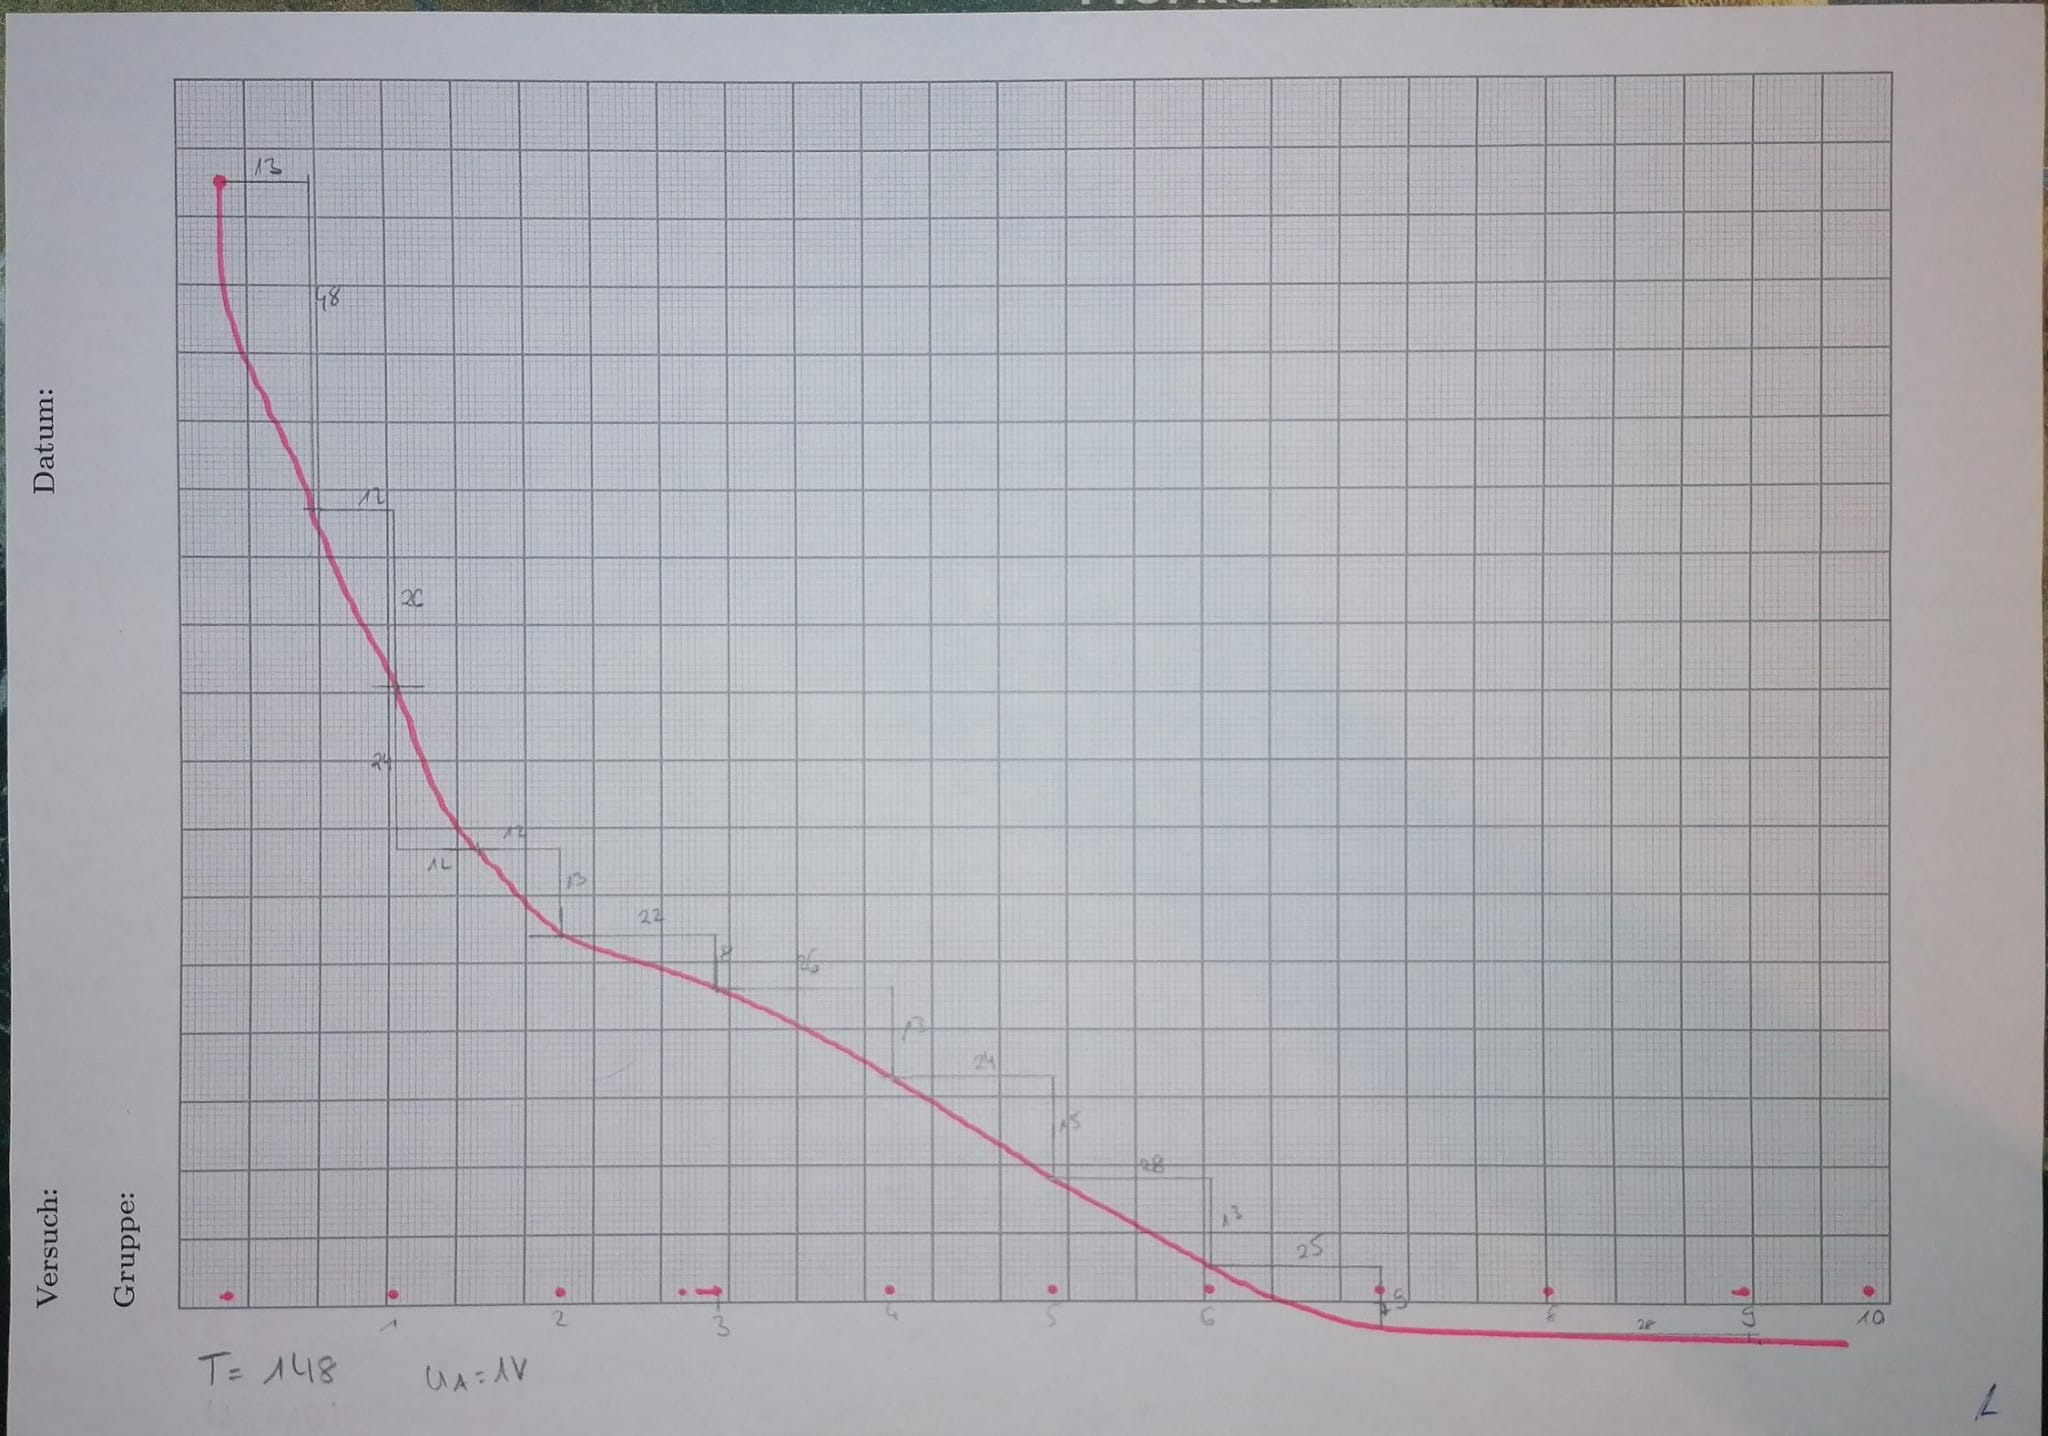
\includegraphics[scale=0.25]{content/Kurve148.jpg}
    \caption{Aufgenommene Messwerte bei $T = 148 \unit{\degreeCelsius}$ und einer Bremspannung von $U_A = \qty{1}{V}$.}
    \label{fig:148}
\end{figure}

\begin{figure}[H]
    \centering
    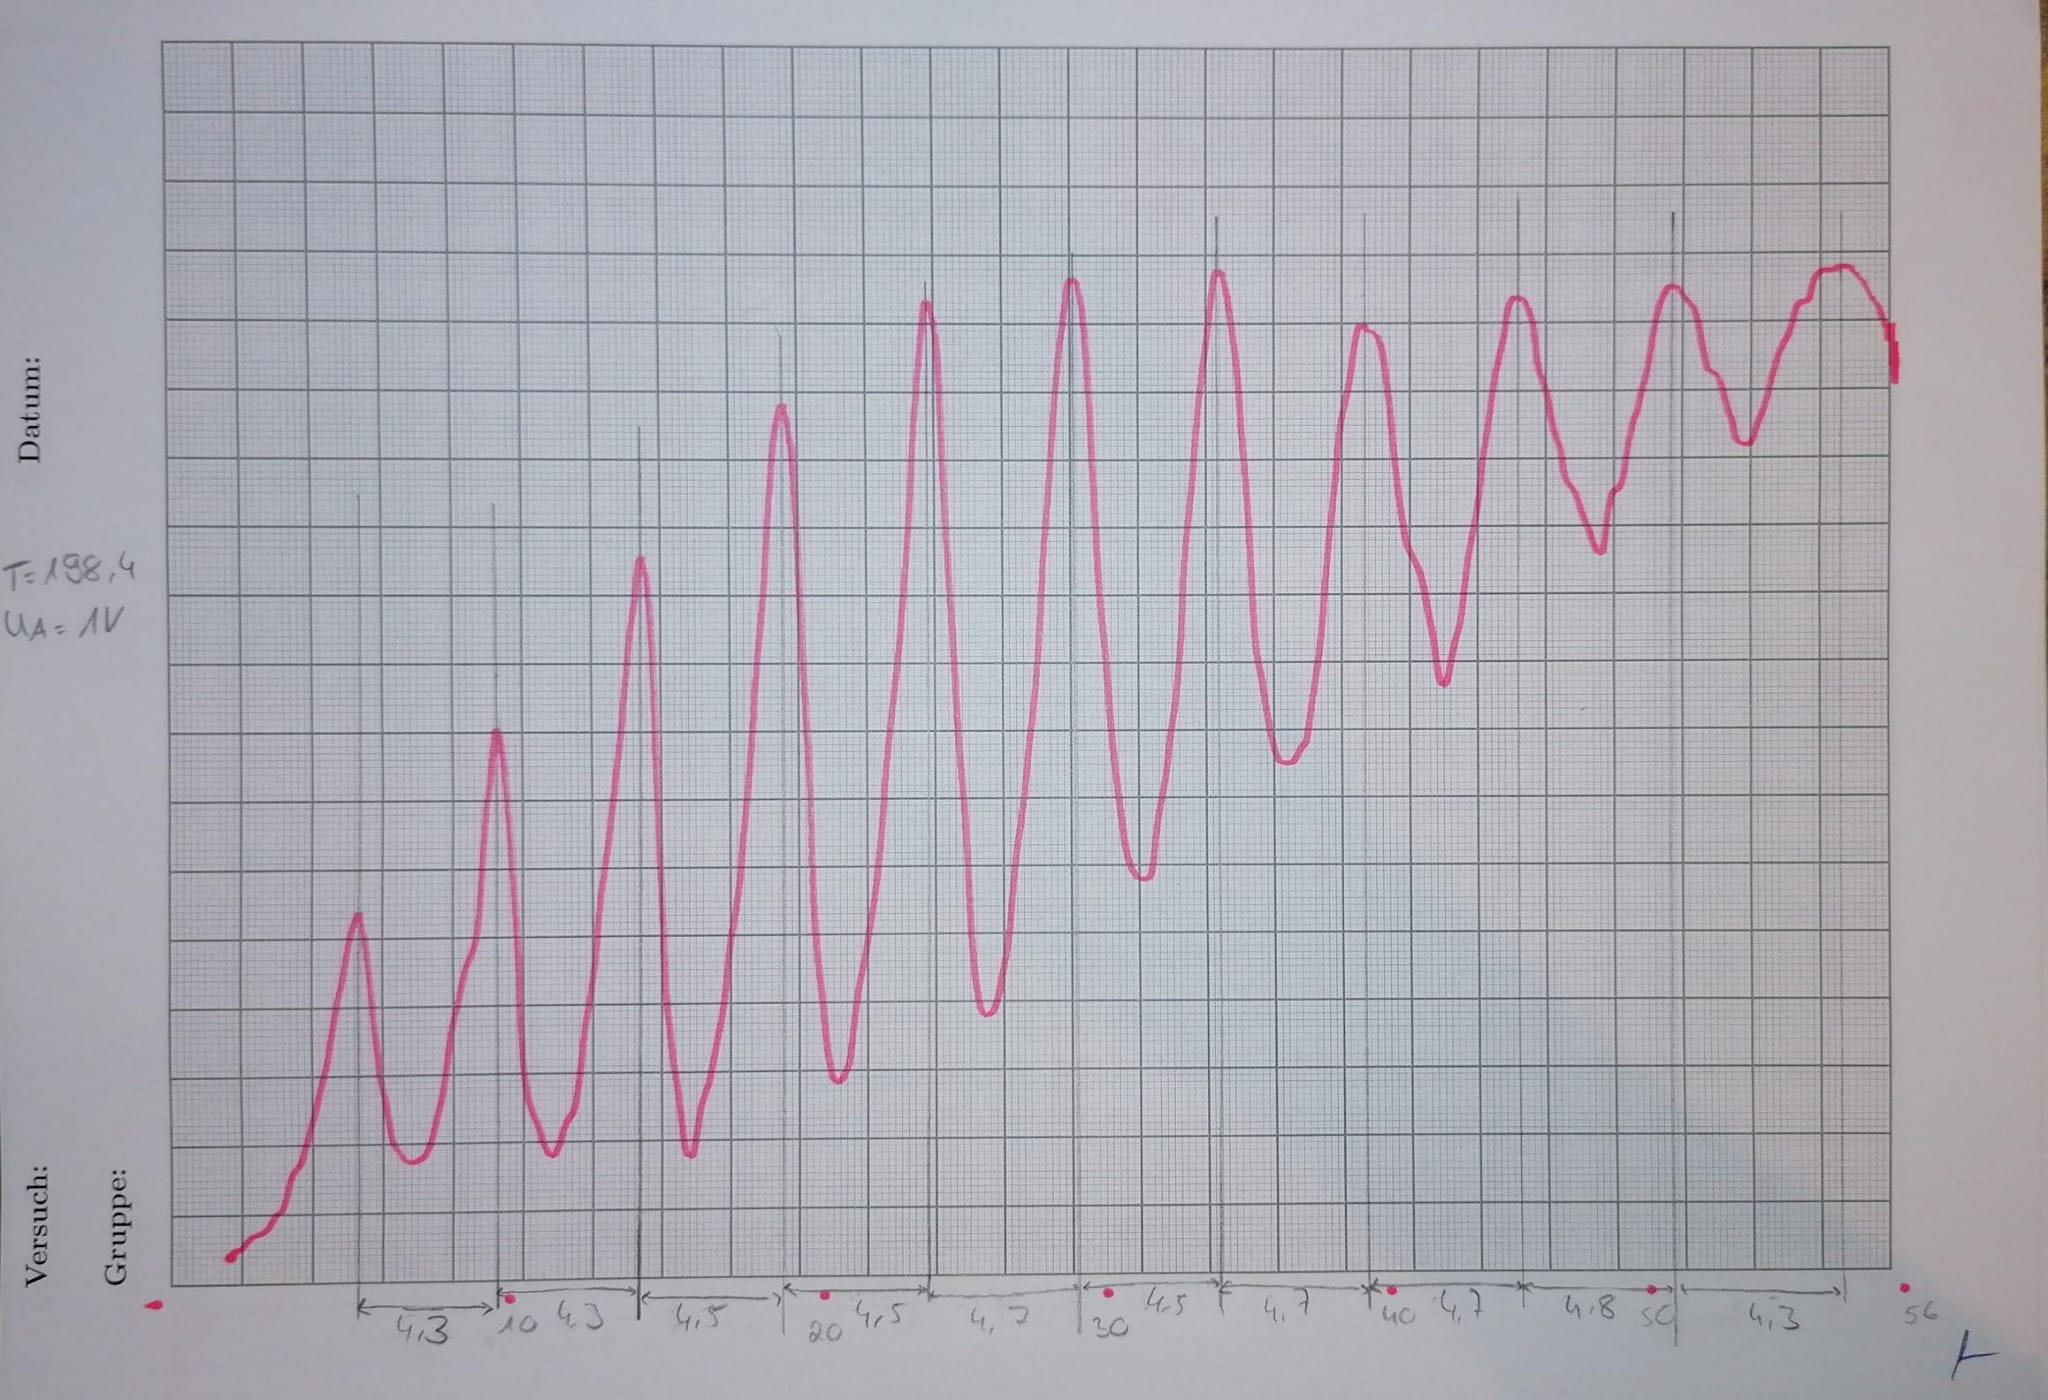
\includegraphics[scale=0.25]{content/Kurve198.jpg}
    \caption{Aufgenommene Kurve bei $T = 198.4\unit{\degreeCelsius}$ und einer Bremspannung von $U_A = \qty{1}{V}$.}
    \label{fig:198}
\end{figure}

\begin{figure}[H]
    \centering
    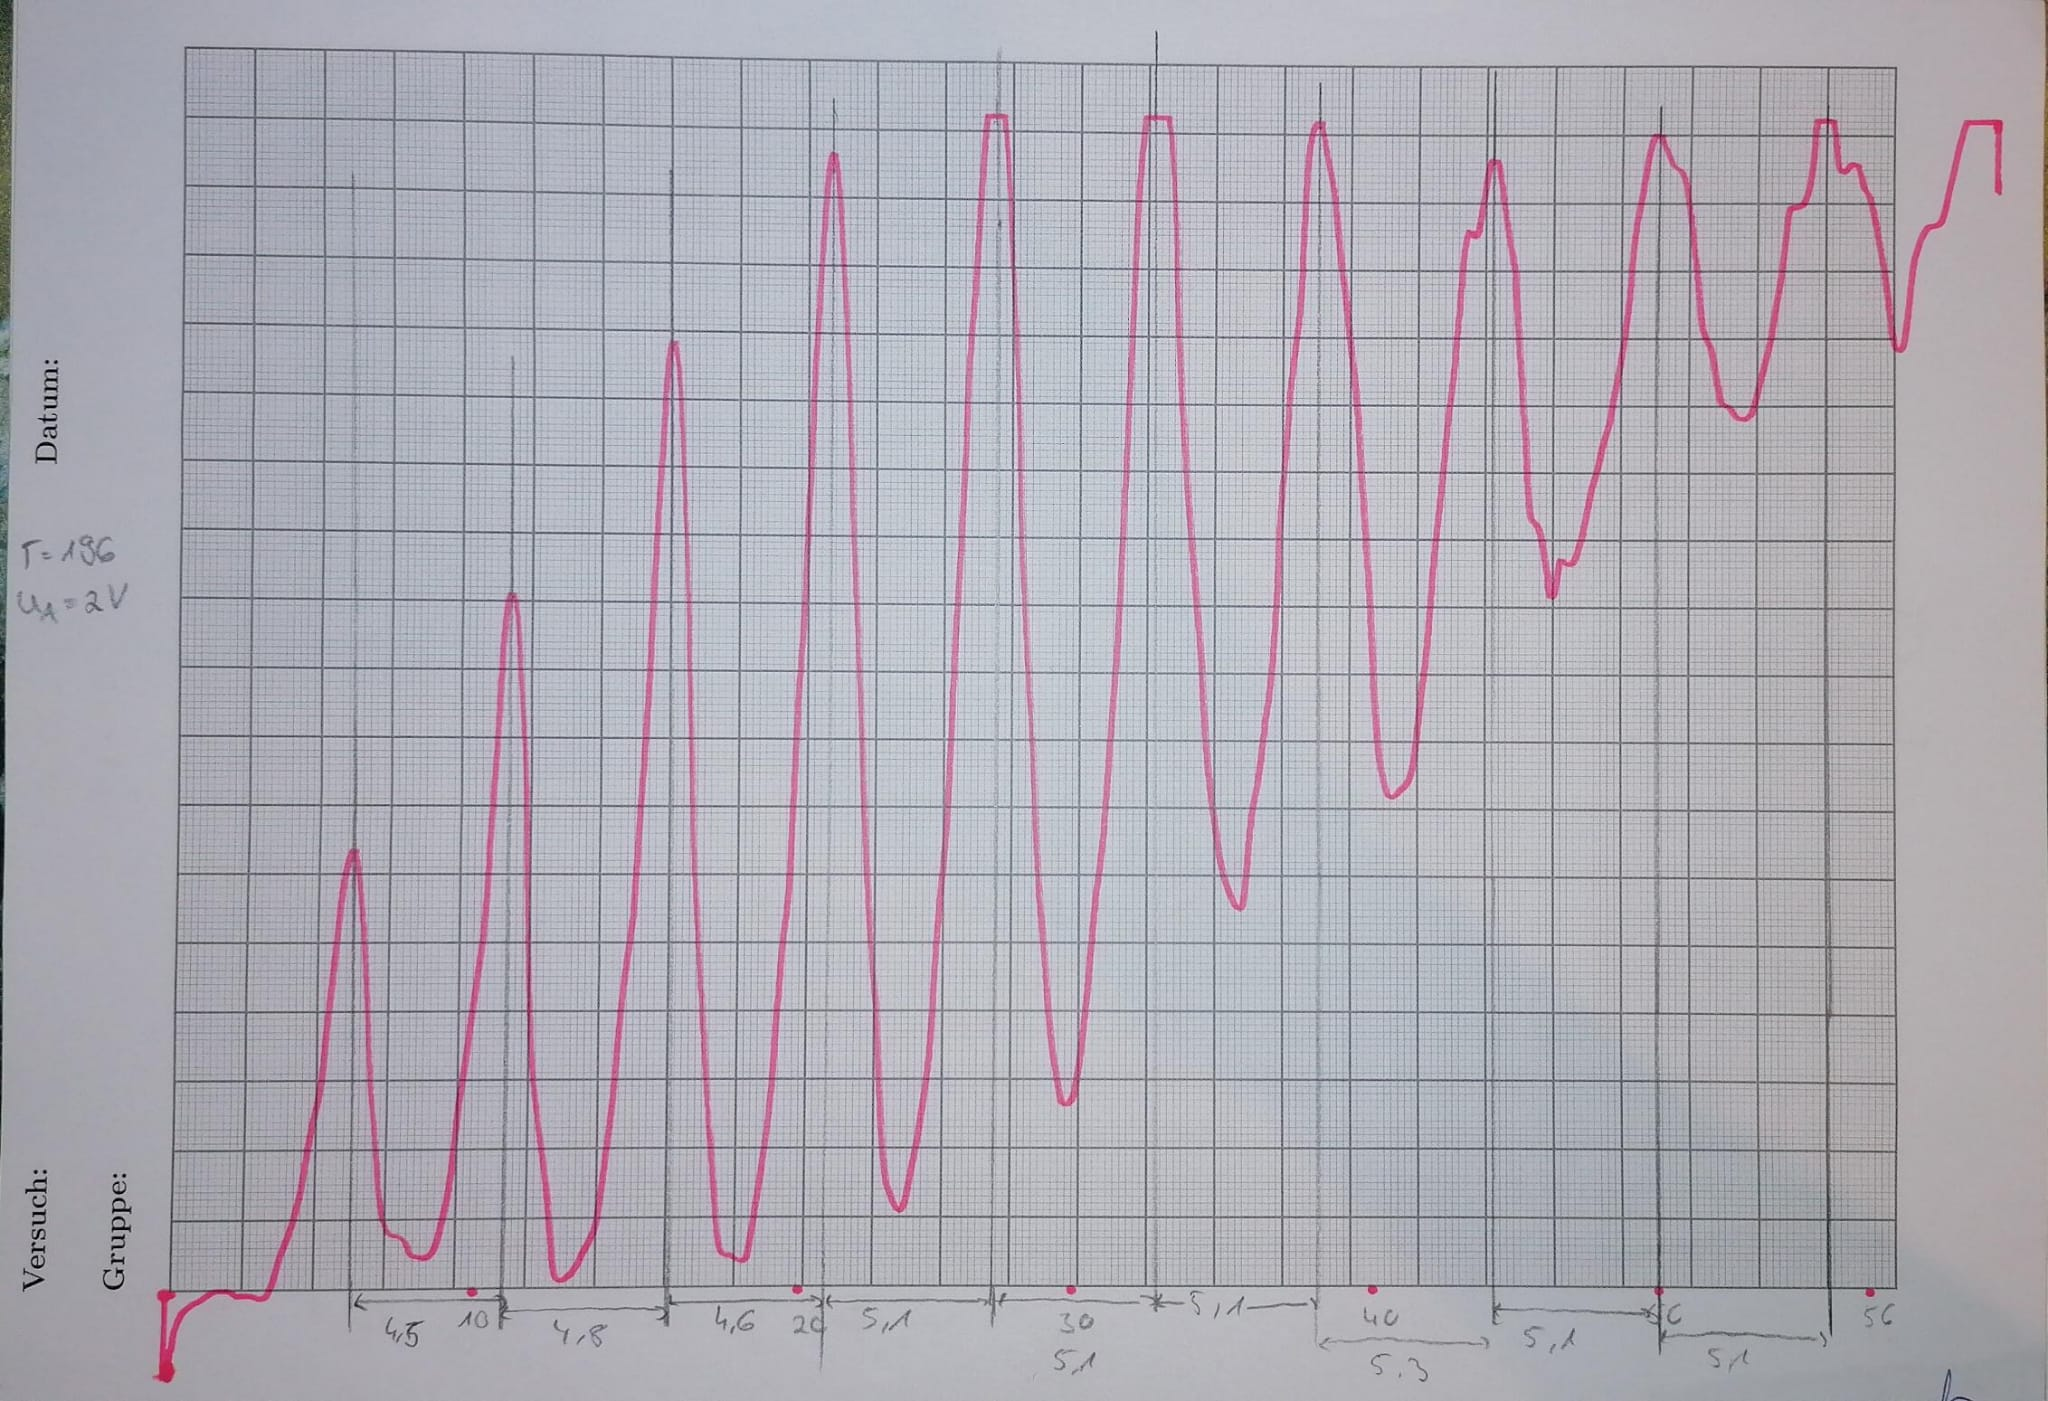
\includegraphics[scale=0.25]{content/Kurve196.jpg}
    \caption{Aufgenommene Kurve bei $T = 196\unit{\degreeCelsius}$ und einer Bremspannung von $U_A = \qty{2}{V}$.}
    \label{fig:196}
\end{figure}

\begin{figure}[H]
    \centering
    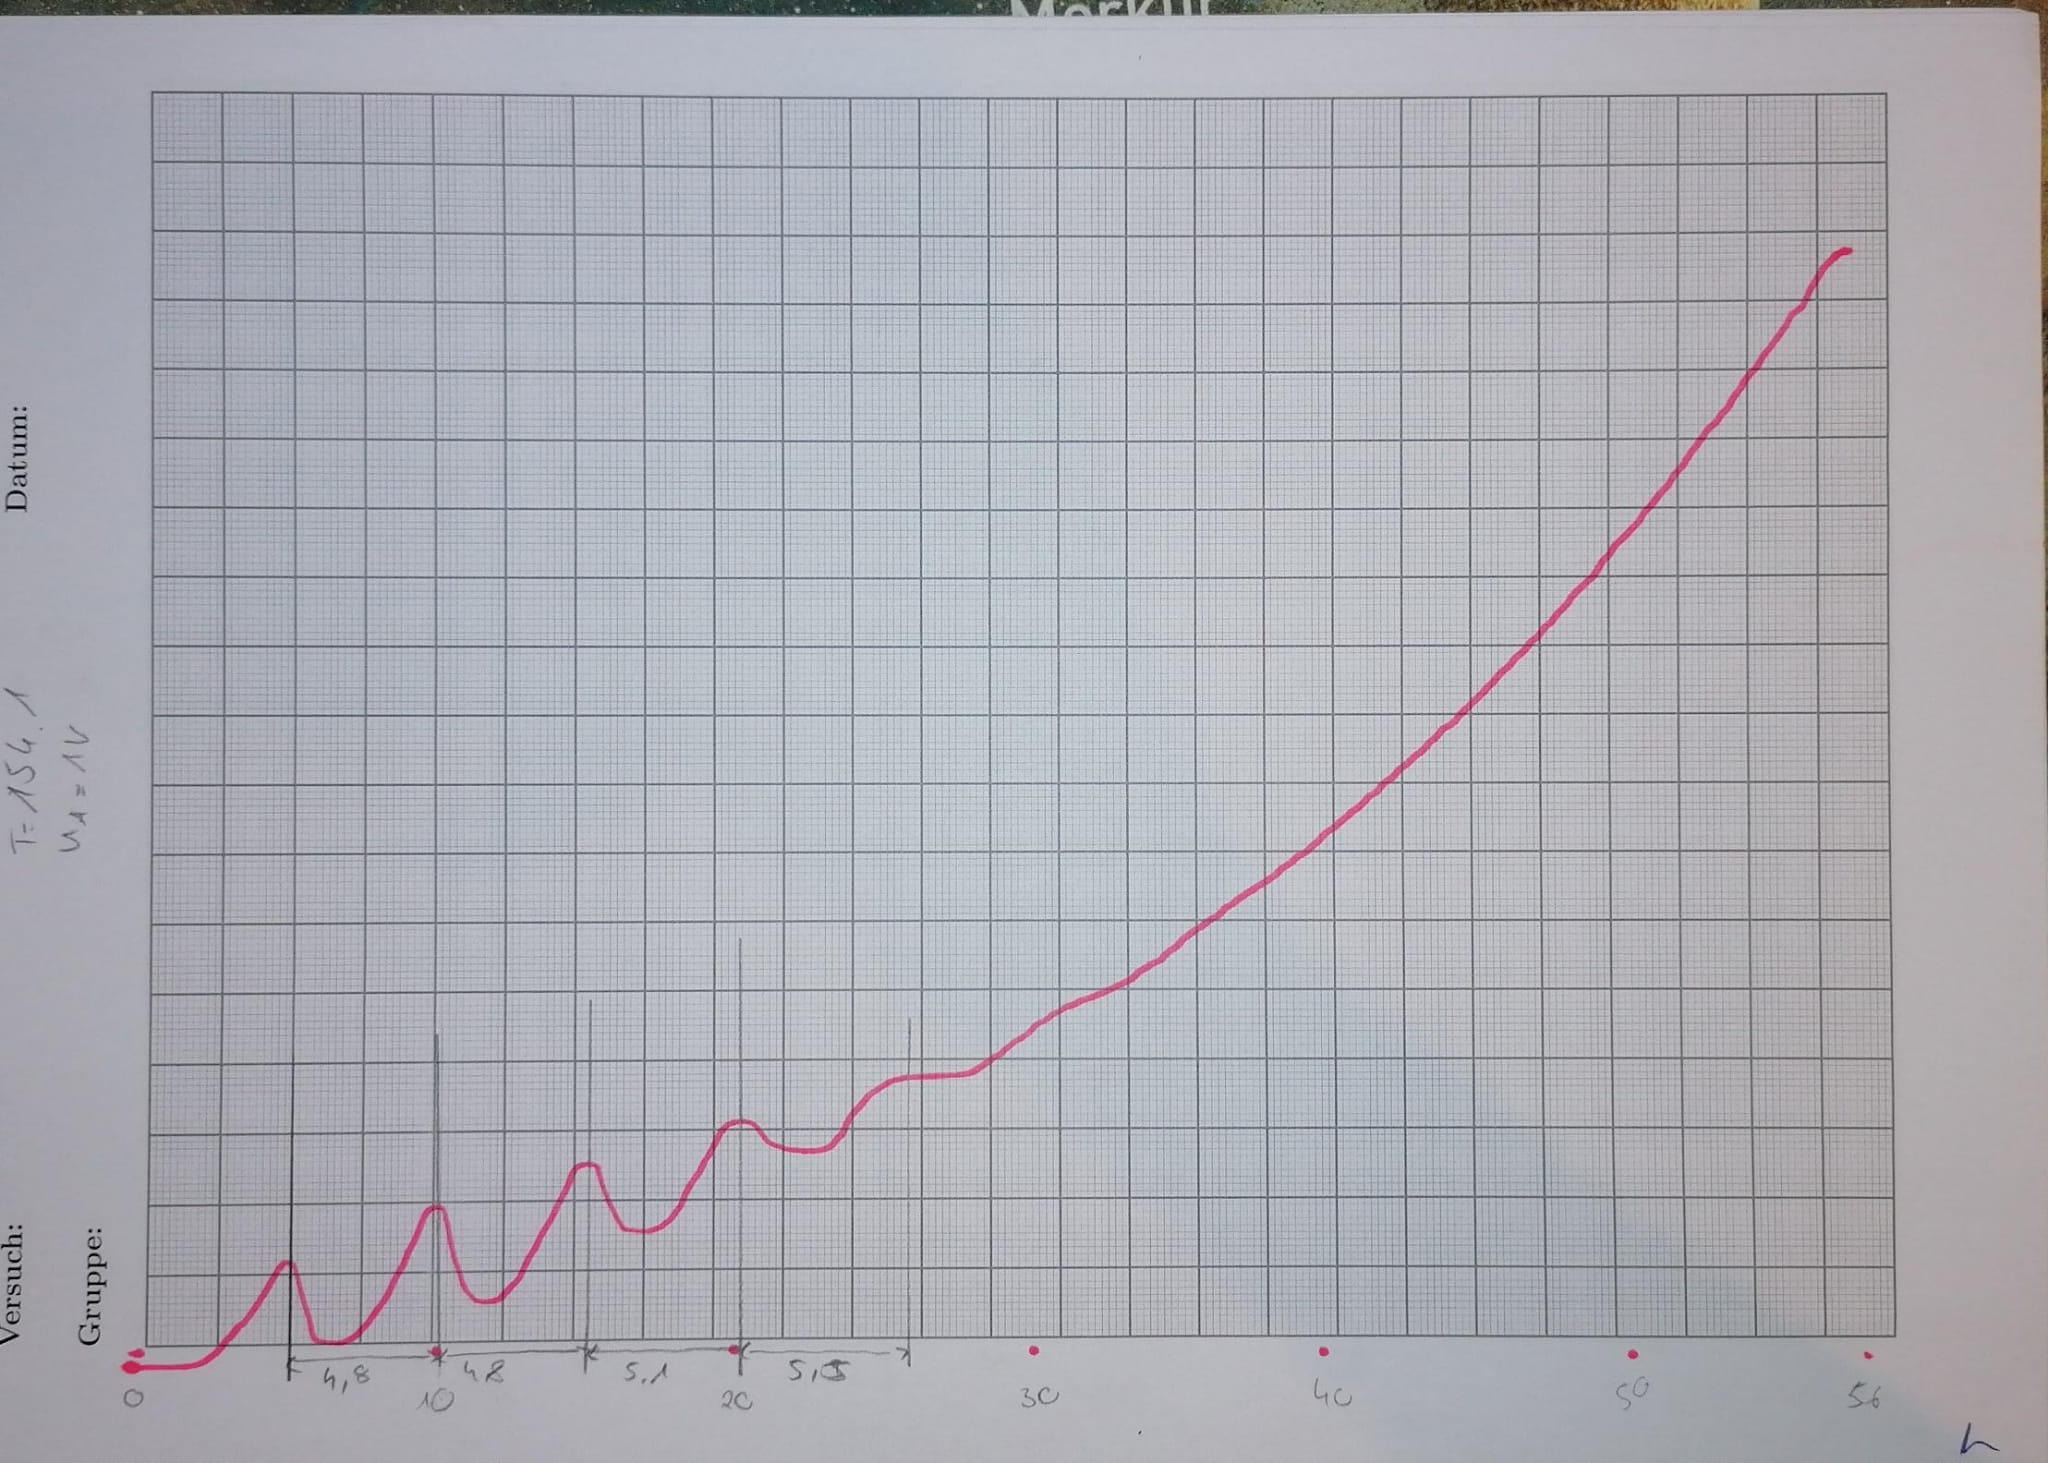
\includegraphics[scale=0.25]{content/Kurve154.jpg}
    \caption{Aufgenommene Kurve bei $T = 154.1\unit{\degreeCelsius}$ und einer Bremspannung von $U_A = \qty{1}{V}$.}
    \label{fig:154}
\end{figure}

\begin{figure}[H]
    \centering
    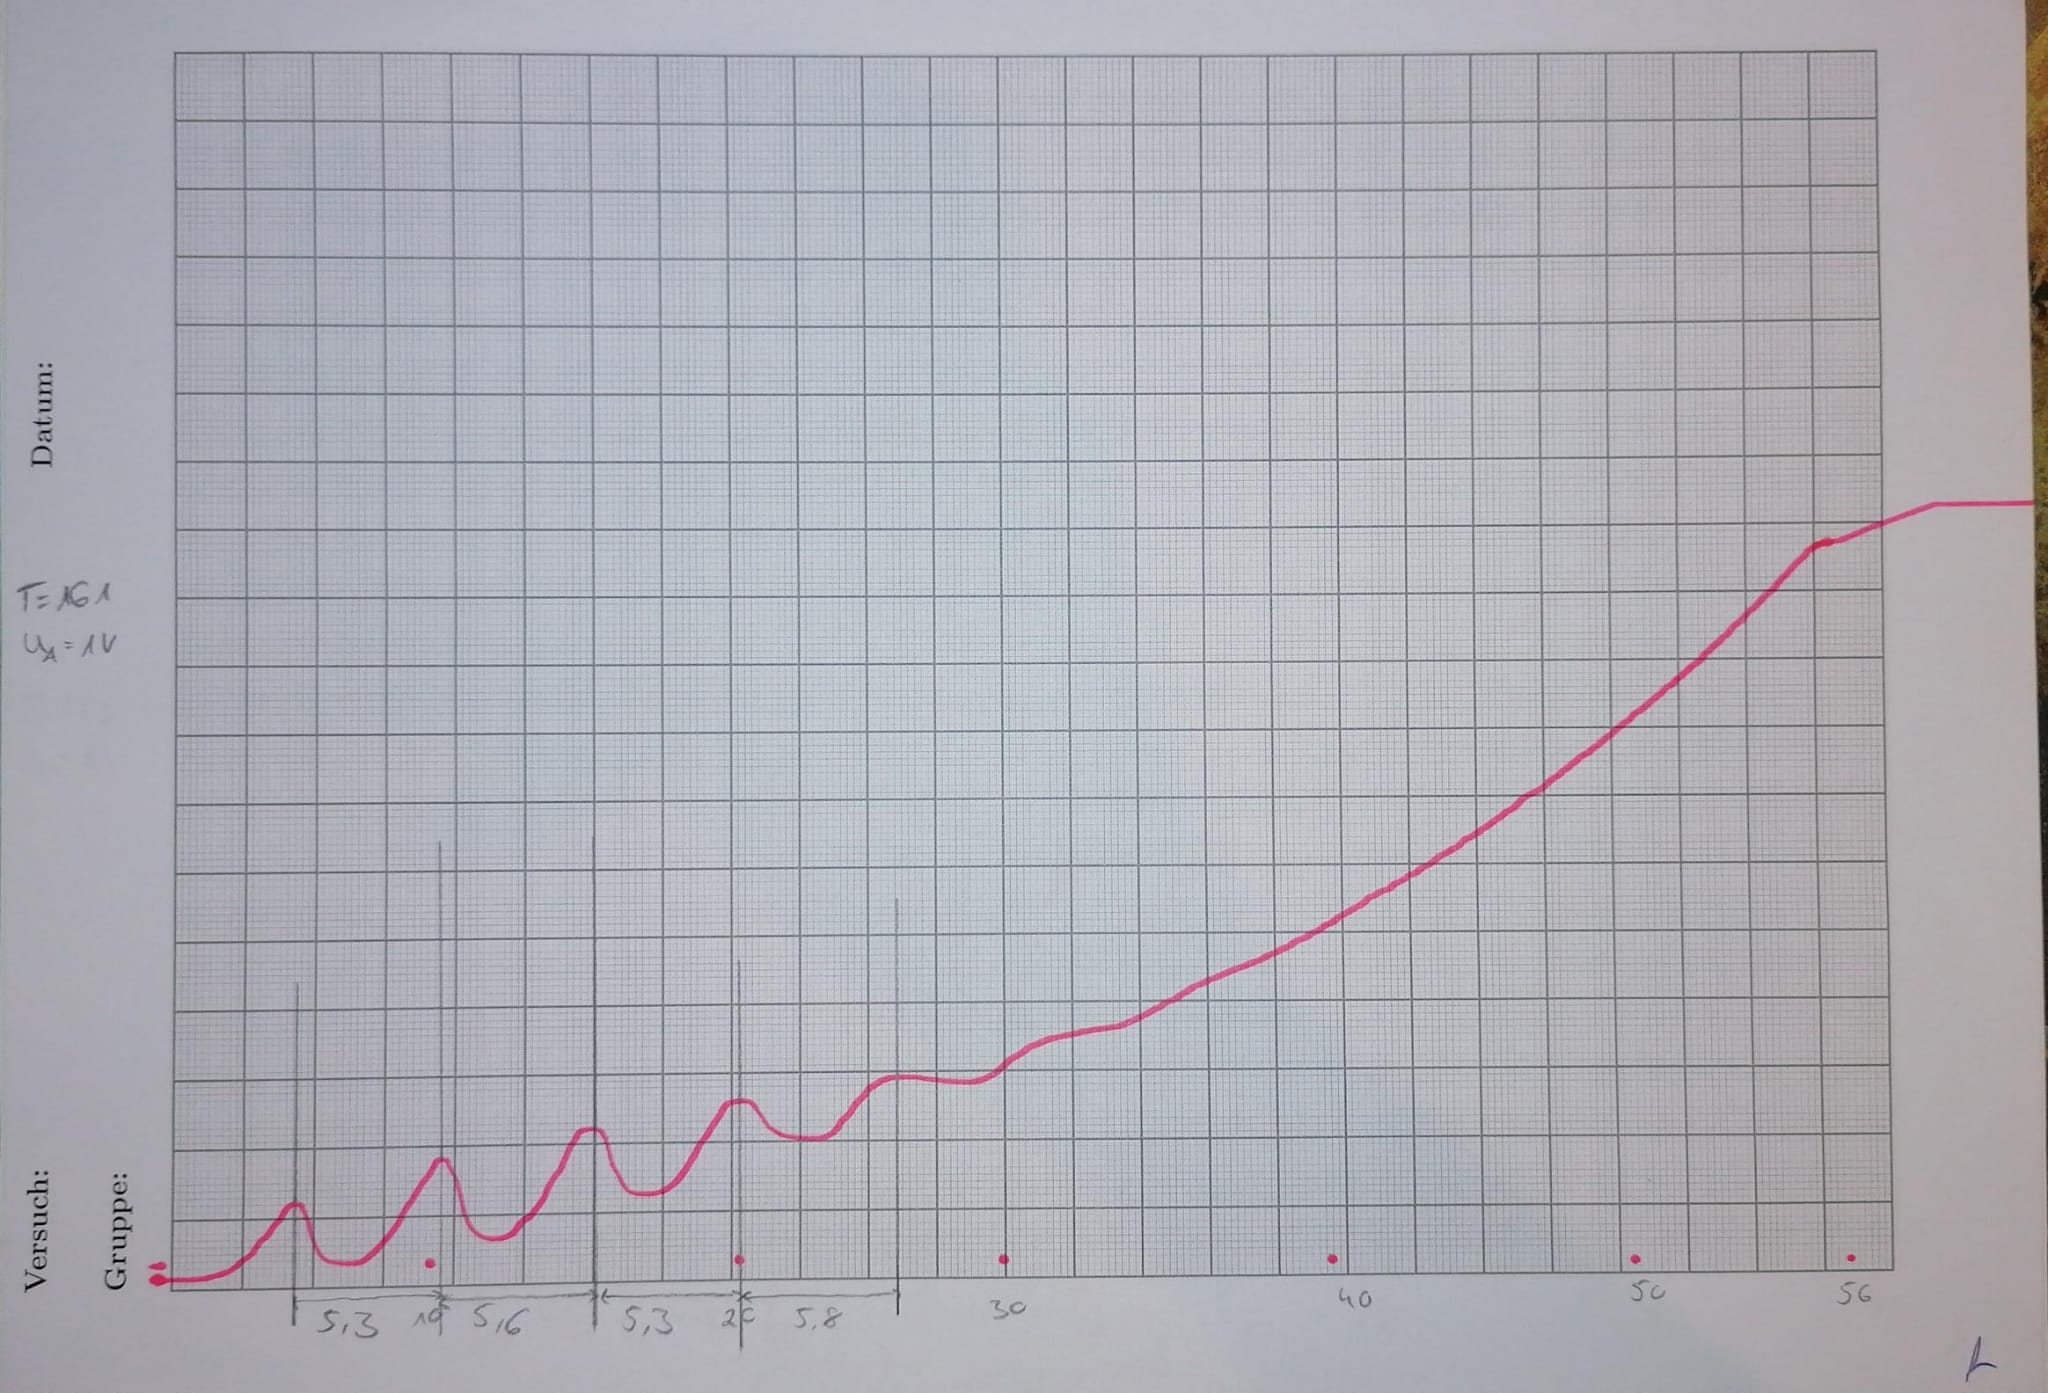
\includegraphics[scale=0.25]{content/Kurve161.jpg}
    \caption{Aufgenommene Kurve bei $T = 161\unit{\degreeCelsius}$ und einer Bremspannung von $U_A = \qty{1}{V}$.}
    \label{fig:161}
\end{figure}

\begin{figure}[H]
    \centering
    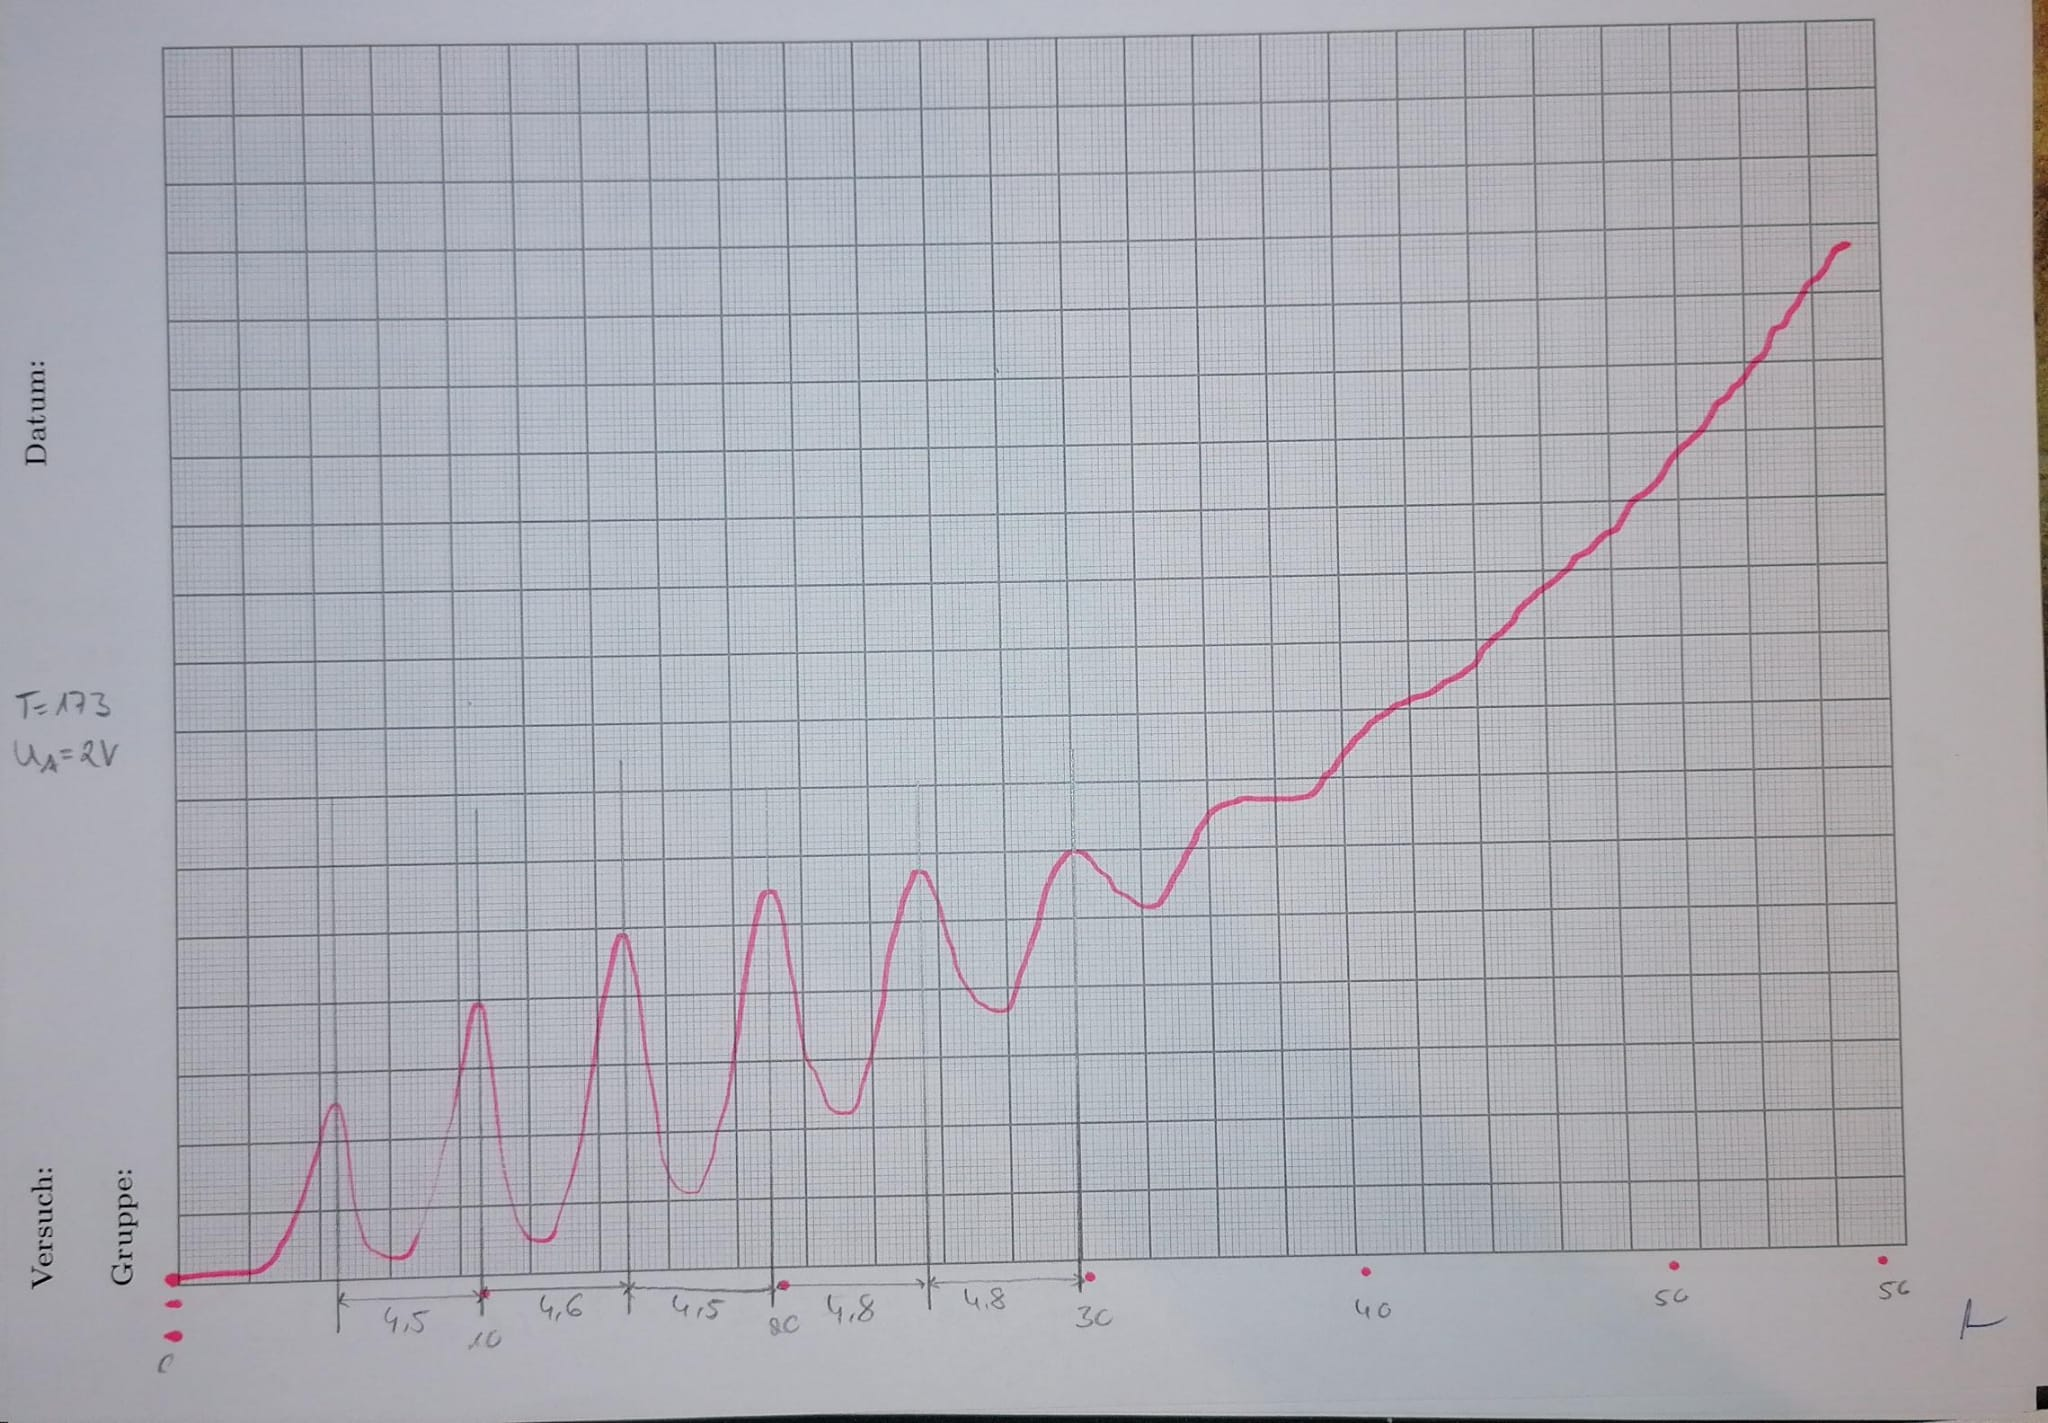
\includegraphics[scale=0.25]{content/Kurve173.jpg}
    \caption{Aufgenommene Kurve bei $T = 173\unit{\degreeCelsius}$ und einer Bremspannung von $U_A = \qty{2}{V}$.}
    \label{fig:173}
\end{figure}

\begin{figure}[H]
    \centering
    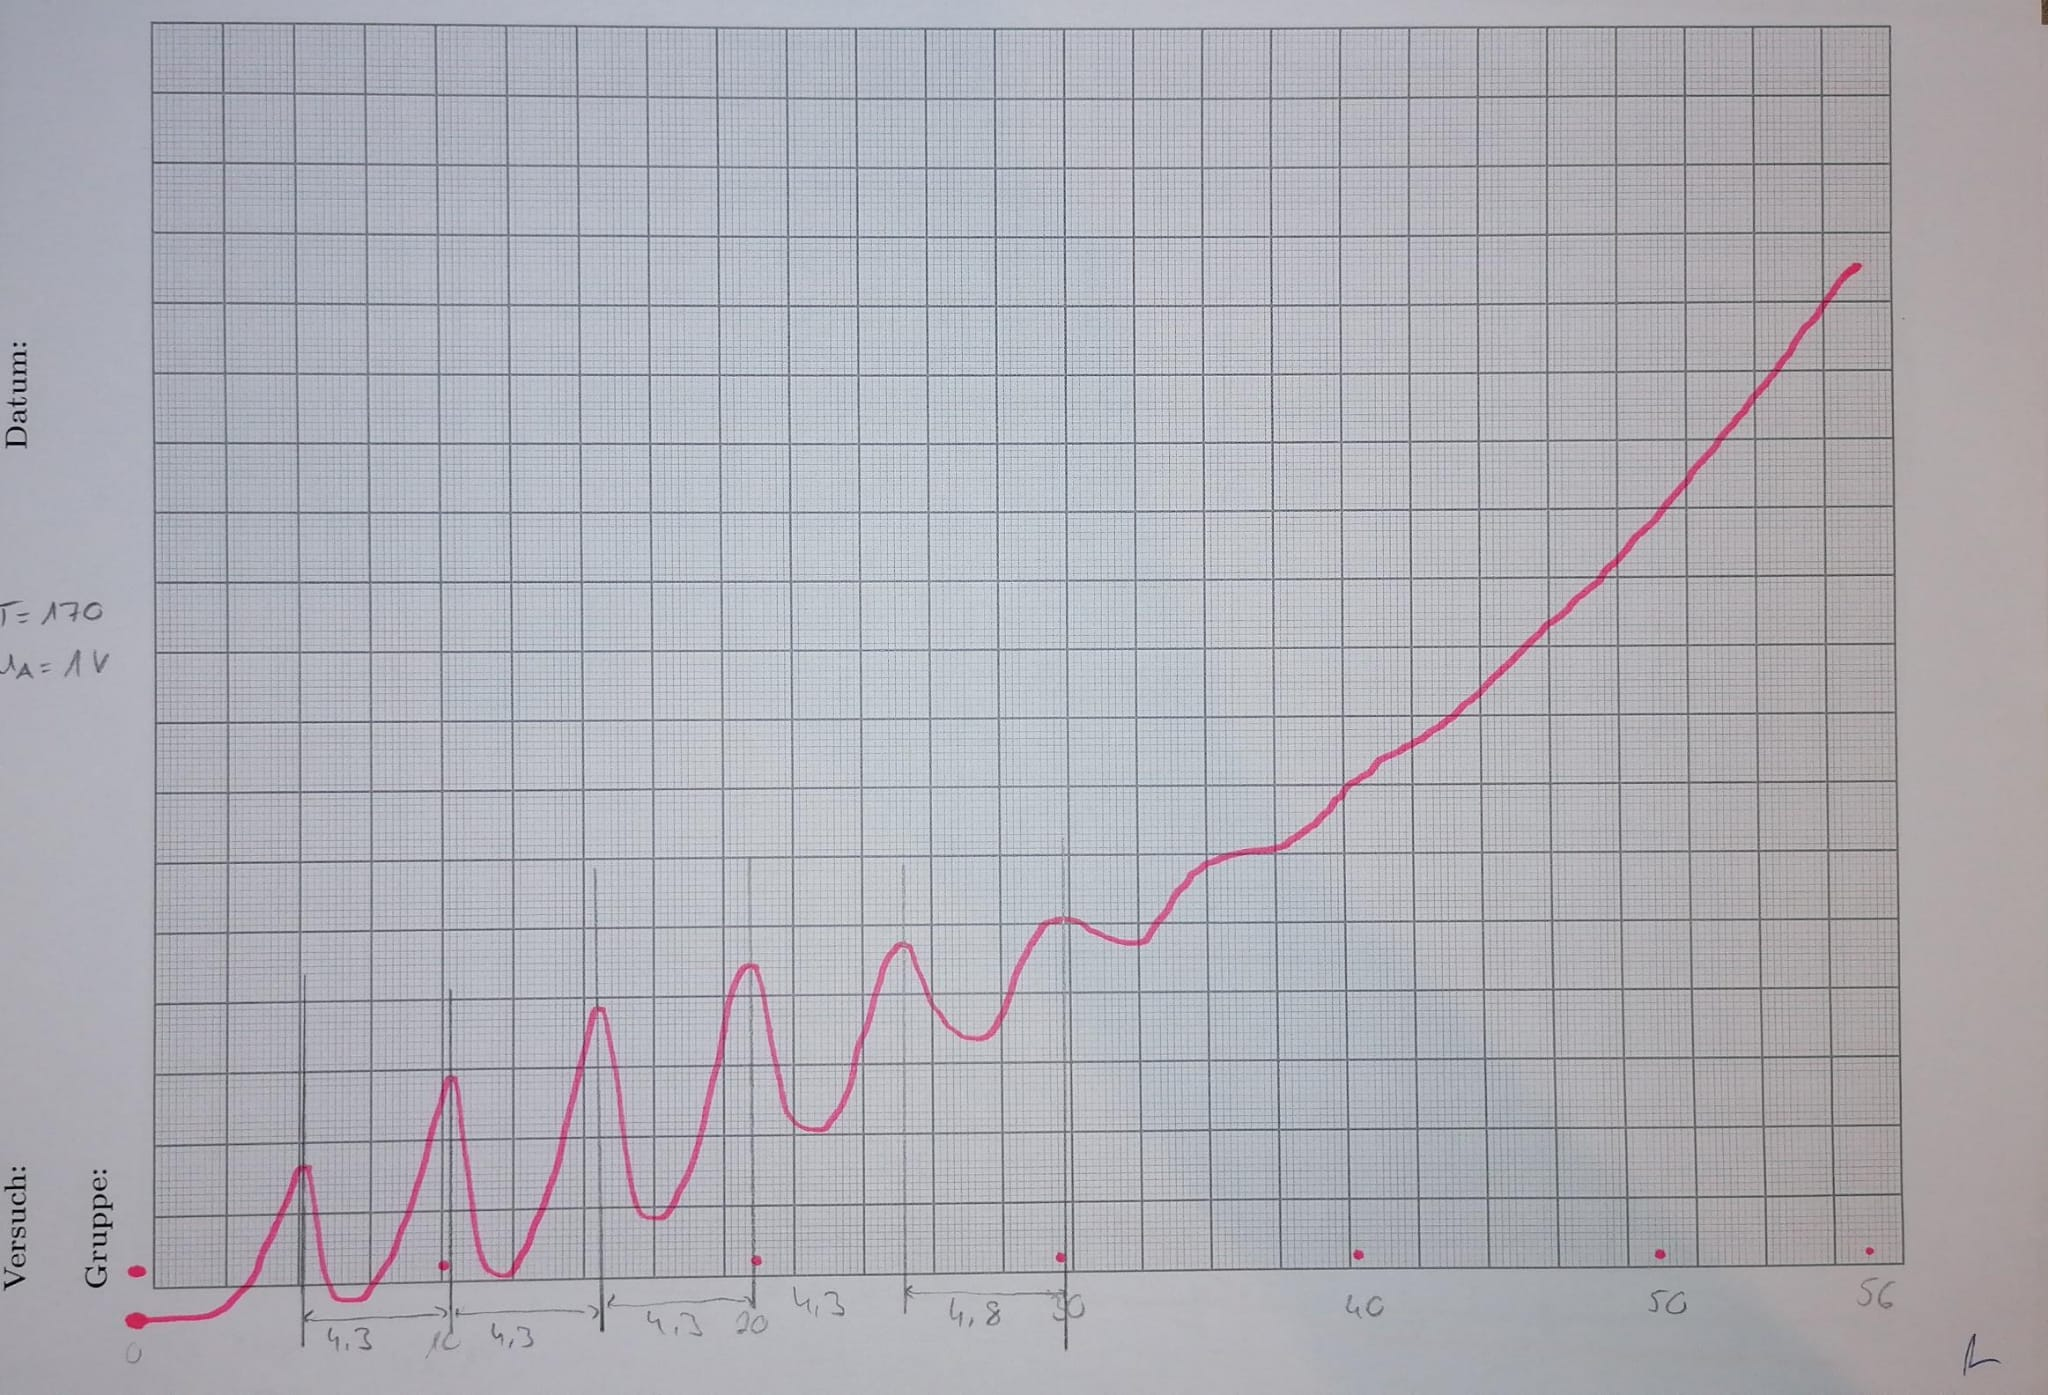
\includegraphics[scale=0.25]{content/Kurve170.jpg}
    \caption{Aufgenommene Kurve bei $T = 170\unit{\degreeCelsius}$ und einer Bremspannung von $U_A = \qty{1}{V}$.}
    \label{fig:170}
\end{figure}